\documentclass[]{llncs}

%% The amssymb package provides various useful mathematical symbols
\usepackage{amssymb}
%% The amsthm package provides extended theorem environments
%\usepackage{amsthm}
\usepackage{amsmath}

%% for url reference
\usepackage{hyperref}
\usepackage{graphicx}

\usepackage{float}
\def\infinity{\rotatebox{90}{8}}

\newcommand{\texp}{|\Delta|}
\newcommand{\block}{\mathcal{B}}
\newcommand{\reward}{\mathcal{W}}
\newcommand{\cost}{\mathcal{C}}
\newcommand*\mean[1]{\bar{#1}}
\newcommand*\widemean[1]{\overline{#1}}

\newcommand{\attackname}{coin-hopping attack}
\newcommand{\AttackName}{Coin-hopping Attack}
\newcommand{\coinA}{$C_1$}
\newcommand{\coinB}{$C_2$}


\begin{document}


\title{[Shote Paper:] Revisiting Difficulty Control for Blockchain Systems}


%\author{authors}
%\institute{institutes}

%\ead{dmitry.meshkov@iohk.io}

\maketitle

\begin{abstract}

The Bitcoin whitepaper~\cite{Nakamoto2008} states that the security of the system is guaranteed as long as honest miners control more than half of the current total computational power. The whitepaper assumes a static difficulty, thus it is equally hard to solve a cryptographic proof-of-work puzzle for any given moment of the system history. However, the real Bitcoin network is using an adaptive difficulty adjustment mechanism.  

In this paper we introduce and analyze a new kind of attack on a mining difficulty retargeting function used in Bitcoin. A malicious miner is increasing his mining profits from the attack, named coin-hopping attack, and, as a side effect, an average delay between blocks is increasing.

We propose an alternative difficulty adjustment algorithm in order to reduce an incentive to perform coin-hopping, and also to improve stability of inter-block delays. Finally, we evaluate the presented approach and show that the novel approach performs better than the original algorithm of Bitcoin.
	
\end{abstract}


\section{Introduction}
\label{sec:intro}

Blockchain systems have attracted significant amount of interest after the Bitcoin whitepaper~\cite{Nakamoto2008} was published in 2008.
Bitcoin security relies on a distributed protocol which maintains a distributed ledger. In the protocol miners are trying to find a partial hash collision in order to generate a valid block by iterating over nonce field values. 
%That is, for a given block $\block$~(with a random nonce included) in order for being valid, the condition $hash(\block) < T$ should hold, where {\em target} parameter $T$ specifies expected hardness of the block generation. This hardness can be also expressed via the {\em difficulty} parameter $D = \frac{1}{T}$.

Alternative systems may rely on other types of computational puzzles rather than finding a partial hash collision, e.g.,~\cite{miller2014permacoin,biryukov2017equihash}. Nevertheless, all of them assume some algorithm that changes the difficulty of the puzzle dynamically. An algorithm for difficulty readjustment is required in order to make an open blockchain system working stable in the face of participants joining and leaving the system (resulting in constantly changing available computational power for solving the puzzles), and also to stabilize mean latency between blocks. 

The difficulty readjustment algorithm in Bitcoin assumes that the total computational power involved in the mining process does not significantly change from epoch to epoch. In contrast, real networks show that a significant variance in computational power happens over long periods.
For example, we show in this paper that due to continuous growth of computational power in the Bitcoin network a mean delay between blocks differs from an expected value by 7\%.
Noteworthy, exponential growth of computational power, often observed in practice, is the absolutely worst case~(regarding the mean block delay divergence) for the Bitcoin's difficulty readjustment algorithm~\cite{kraft2015difficulty}.
 
In this paper we also consider a new type of miner behavior with regards to difficulty readjustment which provides unfair advantage to the miner, and also makes inter-block delays worse. We call the discovered strategy the \attackname{} following the ``pool-hopping'' term raised in~\cite{rosenfeld2011analysis}. In this attack, an adversarial miner is switching from mining one coin to another in the beginning of an epoch, then he is switching back in the beginning of next epoch when difficulty becomes lower. We show how adversarial mining profit is increasing for Bitcoin's difficulty readjustment function, and how inter-block delay suffers from the \attackname{}.

As a solution for the significant variance in computational power and also in order to reduce incentive of the described coin-hopping strategy, we propose an alternative difficulty readjustment procedure. We show that the proposed solution is better suited for exponential growth of the total mining power. It also reduces profit and negative side-effects of the coin-hopping attack.

\subsection{Related Work}

In this section we provide an overview of known formal and informal studies with regard to the dynamic nature of the difficulty parameters in Bitcoin. Following the well known paper of Garay et al.~\cite{garay2015bitcoin}, generalizing the Bitcoin backbone protocol in a static difficulty setting, a newer paper from the same authors~\cite{gkl16} is providing a positive answer on whether basic security properties of the Bitcoin backbone protocol~(common prefix, chain quality and chain growth) hold in case of dynamic difficulty, in a cryptographic setting with an arbitrary adversary. Nevertheless, studying concrete attacks against the real protocol is still needed.      

The Timejacking attack~\cite{timejacking2011} allows an attacker to first shift the network time at a victims node~(which is calculating network time by averaging timestamps it gets regularly from neighbors) and then force the victim node to reject a block with a specially crafted timestamp~(other nodes are accepting). The time wrapping attack~\cite{artforz2011} is exploiting the fact that Bitcoin is using difference in timestamps between last and first block in an epoch, instead of the last block in an epoch and last block in a previous epoch. By using specially crafted timestamps for the last block of each epoch, an attacker can produce more blocks for a time window with more work contributed to his chain. The difficulty raising attack, introduced in~\cite{bahack2013theoretical}, allows an attacker to discard $n$-depth block, for any $n$, and for any computational power of the attacker, with probability 1 if he is willing to wait long enough.

Another paper~\cite{kraft2015difficulty} is introducing an alternative difficulty readjustment function designed to work better than Bitcoin's not just for almost constant mining power but also when the power is growing exponentially with time. We provide comparison with this function in the paper in one of the following sections.  

The paper is organized as follows: in Section~\ref{sec:bit} we provide a detailed view of Bitcoin's readjustment function. In Section~\ref{sec:attack} we introduce the coin-hopping attack, followed by the definition of an improved difficulty readjustment function described in section~\ref{sec:improved}. Section~\ref{sec:sim} provides results of evaluation of the presented approach. 

\section{Bitcoin Mining}
\label{sec:bit}

The concept of Bitcoin mining was introduced in Section 4 of the Bitcoin whitepaper~\cite{Nakamoto2008}, and then discussed in detail in the papers~\cite{kraft2015difficulty},\cite{gkl16}. Bitcoin miner generates a block by iterating over a {\em nonce} value and calculating the hash of a block with the nonce value included. For a block $\block$ to be valid, a value of a hash function has to be less than the current {\em target} $T$, $hash(\block) < T$, where $hash$ is an ideal cryptographic hash function. Hardness to find a block could be expressed also via {\em difficulty} $D$ as $D = \frac{1}{T}$. If output of the $hash$ function is $\mu$ bits long then the probability to generate a block by doing $q$ requests to the hash function is $\frac{T \cdot q}{2^\mu} = \frac{q}{D \cdot 2^\mu}$. We define miner's {\em hashrate} $R$ as $R = \frac{q_s}{2^\mu}$, where $q_s$ is number of queries done by miner $s$ per time unit. The probability to generate a block within a time unit is then $\frac{R}{D}$. In our analysis we assume that number of blocks mined over  long period of time is proportional to hashrate of a miner. However, there are known strategies to mine a disproportionally high number of blocks, such as~\cite{selfish}, and the strategies are in correspondence with a general result in~\cite{garay2015bitcoin}, which is introducing {\em chain quality property}. The property sets an upper bound on number of blocks an adversary can generate over a sufficiently long period, however, this number can be higher than the relative hashrate of the adversary; the result got under an assumption of static difficulty. Adversarial manipulations with difficulty can be combined with selfish mining and other strategies to achieve disproportionally high number of blocks, making previous results worse, but this is out of scope of this paper: here, we study manipulations with difficulty in isolation. 


Every $M$ blocks ($M = 2016$ for Bitcoin) the difficulty is recalculated as
\begin{equation}
D_{i+1}=D_i \cdot {M \cdot \texp \over S_m}
\end{equation}
where $\texp$ is the expected time interval between blocks and $S_m$ is the actual time spent to generate $M$ blocks.
For the Bitcoin network, the observed time interval of $\approx${\em 9 minutes 20 seconds} is less than the planned value of $\texp = 10$ {\em minutes} due to continuous growth of the computational power of the network.
Difficulty recalculation interval $M=2016$ has been chosen to recalculate difficulty every 2 weeks on average.
The epoch length is big enough to see the computational power of the network being changing over it: mean delay is close to the planned 10 minutes right after target recalculation, whereas at the end of an epoch it is less than 9 minutes in average.

The next section describes an attack against the recalculation algorithm.

\section{\AttackName}
\label{sec:attack}

We consider the following attack involving an adversarial miner $\mathcal{A}$:

\begin{itemize}
\item There are at least 2 possible coins (\coinA{},\coinB{}) $\mathcal{A}$ can contribute to. Without a loss of generality, we assume that each of them provides about the same profitability of the mining activity.
\item $\mathcal{A}$ is mining coin \coinB{} before the beginning of an epoch $A$. At the beginning of $A$ he is switching to mine coin \coinA{}.
\item Without the contribution of miner $\mathcal{A}$ the total mining power of the \coinB{} network for the epoch decreases.
\item For an epoch $B$ right after epoch $A$, the difficulty of \coinB{} is to be readjusted to a lower value. So $\mathcal{A}$ starts mining \coinB{} again with a lower difficulty.
\end{itemize}

We call this strategy a {\em \attackname{}}.

To calculate the profit the adversarial miner gains from this attack, we use Bitcoins' difficulty recalculation function and assume a  constant network hashrate (with respect to the rest of the network, without the adversarial miner).
We denote the hashrate of miners not participating in the coin-hopping attack as $R_0$ in both \coinA{} and \coinB{}, and we denote the hashrate of the adversarial miner as $R_a=R_0\cdot p, 0 < p < 1 $.
Before epoch $A$ the adversary is mining coin \coinB{}, thus the difficulty of the \coinB{} network  is $D_0 = (R_0+R_a) \cdot \texp$~(see Section 3.1 in~\cite{kraft2015difficulty}).
During the epoch A the difficulty of the \coinB{} network is still $D_0$, and $\mathcal{A}$ switches to mine coin \coinA{} at a difficulty $D_1 = R_0 \cdot \texp$  calculated from honest miners hashrate $R_0$ only.
During the epoch B the adversary starts mining of \coinB{}, now at difficulty $D_1$, while honest miners on chain \coinA{} continue to mine it with higher difficulty $D_0$.
After that $\mathcal{A}$ continues to switch between chains \coinA{} and \coinB{} always mining on the chain with lower difficulty $D_1$, spending $R_0 \cdot \texp$ computational power per block, whereas honest miners spend $(R_0+R_a) \texp$ computational power per block.

Every epoch honest miners with hashrate $R_0$ will generate $M \cdot R_0 \over R_0 + R_a$, blocks, whereas $\mathcal{A}$ will generate $M \cdot R_a \over R_0$ blocks.
If $\reward$ is block reward, the additional profit of the adversary is calculated as the difference of what he mines based on the lower difficulty in contrast to the difficulty he would mine at without hopping between the coins:
\begin{equation}
\begin{aligned}
{\reward \cdot M \cdot { R_a \over R_0} - \reward \cdot M \cdot { R_a \over R_0 + R_a}}  
%= {\reward \cdot M \cdot ( { R_a \over R_0} - {R_a \over R_0 + R_a})} = \\
%= {\reward \cdot M \cdot { R_a \cdot (R_0 + R_a) + R_a \cdot R_0 \over R_0 \cdot (R_0 + R_a) }} = \\
= {\reward \cdot M \cdot { R_a^2 \over R_0 \cdot (R_a + R_0) }} = \\
= {\reward \cdot M \cdot {R_0^2 \cdot p^2 \over R_0 \cdot (R_0 \cdot p + R_0)}} 
= {\reward \cdot M \cdot { p^2 \over 1+p }}
\end{aligned}
\end{equation}

Remarkably, under such an attack the mean time between blocks in both chains \coinA{} and \coinB{} will be
\begin{equation}
\label{eq:ati}
{T_a={T\over 2}({R_0+R_a\over R_0} + {R_0 \over R_0+R_a}) = T(1 + {p^2\over 2(1+p)})}
\end{equation}
which is bigger than the planned time $T$.

%The next section provides a new algorithm for difficulty adjustment.

\section{Improved Difficulty Adjustment}
\label{sec:improved}

The difficulty adjustment algorithm employed by Bitcoin works as designed: if the hash rate of the network is constant, it yields to the desired block rate. However it does not achieve the desired block rate in other situation, and is vulnerable to the attack described in \ref{sec:attack}.
In this section we propose an alternative difficulty adjustment algorithm.

First, we state properties of an ideal difficulty update algorithm:
\begin{enumerate}
\item{It should be resistant to known types of attacks based on difficulty manipulation.}
\item{It should lead to an almost constant desired block rate for random fluctuations in the network hashrate.}
%\item{It should be simple enough to use integer arithmetic for all computational steps.}
\end{enumerate}

%Security is the most important feature of blockchain systems and should be regarded with highest priority.
%Incorrect block rate is not considered a big problem in the Bitcoin community but it may be important for more advanced applications of blockchain systems.
%Implementation of the \textit{ideal} difficulty update algorithm based solely on integer arithmetics is desired for a platform independent approach.
%This rule is not required necessarily, since as mentioned in \cite{kraft2015difficulty}, it is possible to include non-integer algorithm parameters as part of the block, but it provides another way of difficulty manipulating to an attacker.

We propose a difficulty adjustment algorithm based on the well-known linear least squares method\cite{lawson1974solving}, we name it {\em linear algorithm}. In the simplest case of pair linear regression $y=kx+b$, coefficients may be calculated as follows:

\begin{equation}
  \begin{cases}
    k= {{\widemean{xy} - \mean{x} \mean{y}} \over {\widemean{x^2} - \widemean{x}^2}}  \\
    b= \widemean{y}-k\widemean{x}
  \end{cases}
\end{equation}

Difficulty of the $i-th$ epoch $D_i$ can be caclulated from the observed difficulties of previous $N$ epochs $D_{i-1},...,D_{i-N}$ as follows:

\begin{equation}
  \begin{cases}
    k= {2\sum_{n=i-N}^{i-1} (D_n \cdot n) - (2i-N-1)\cdot \sum_{n=i-N}^{i-1} D_n \over N ( (i-N)^2 + (i-1)^2 + (2i-N-1)^2/2 )} \\
    b= \sum_{n=i-N}^{i-1} D_n / N-k (2i-N-1)/2 \\
    D_i= k \cdot i + b
  \end{cases}
\end{equation}

Note that for accurate difficulty prediction we use $N$ last observed difficulties, rather than just one, as implemented in Bitcoin, but it is still possible to use this algorithm right after the second epoch of the history.


% We regard it as the good candidate for difficulty update algorithm, because:
% \begin{enumerate}
% \item{It should reduce profit of the attack, described in Section~\ref{sec:attack}. Calculations of the attacker profit are described in Section~\ref{sec:sim}}
% \item{It leads to desired block rate for linear changes in the hash rate.
% This means, that regarding block rate, linear algorithm is better than one of Bitcoin in all cases, except constant hash rate, when both provide the same result. }
% \item{It is simple enough to use integer arithmetic for all computational steps with high fidelity.}
% \end{enumerate}

The next section provides an evaluation of the linear algorithm.

\section{Evaluation}
\label{sec:sim}

We now present simulation results that show that the  method proposed in Section~\ref{sec:improved} outperforms Bitcoin's difficulty update algorithm.
We will regard difficulty growth in this section, keeping in mind the fact, that it is closely related with network hash rate, which is usually considered in literature.

\subsection{Exponential Difficulty Growth}
\label{sec:experiment}
First, we observe exponential difficulty growth as it occures in practice in the Bitcoin network. Exponential difficulty growth is the absolutely worst case possible for Bitcoin~\cite{kraft2015difficulty}.
For simplicity, we consider a situation where network hashrate is increasing by 10\% each epoch~(more complicated research of exponential difficulty growth can be found in~\cite{kraft2015difficulty}).
Figure~\ref{fig:exp} presents how Bitcoin and linear algorithms perform over epochs.

\begin{figure}[h]
\center{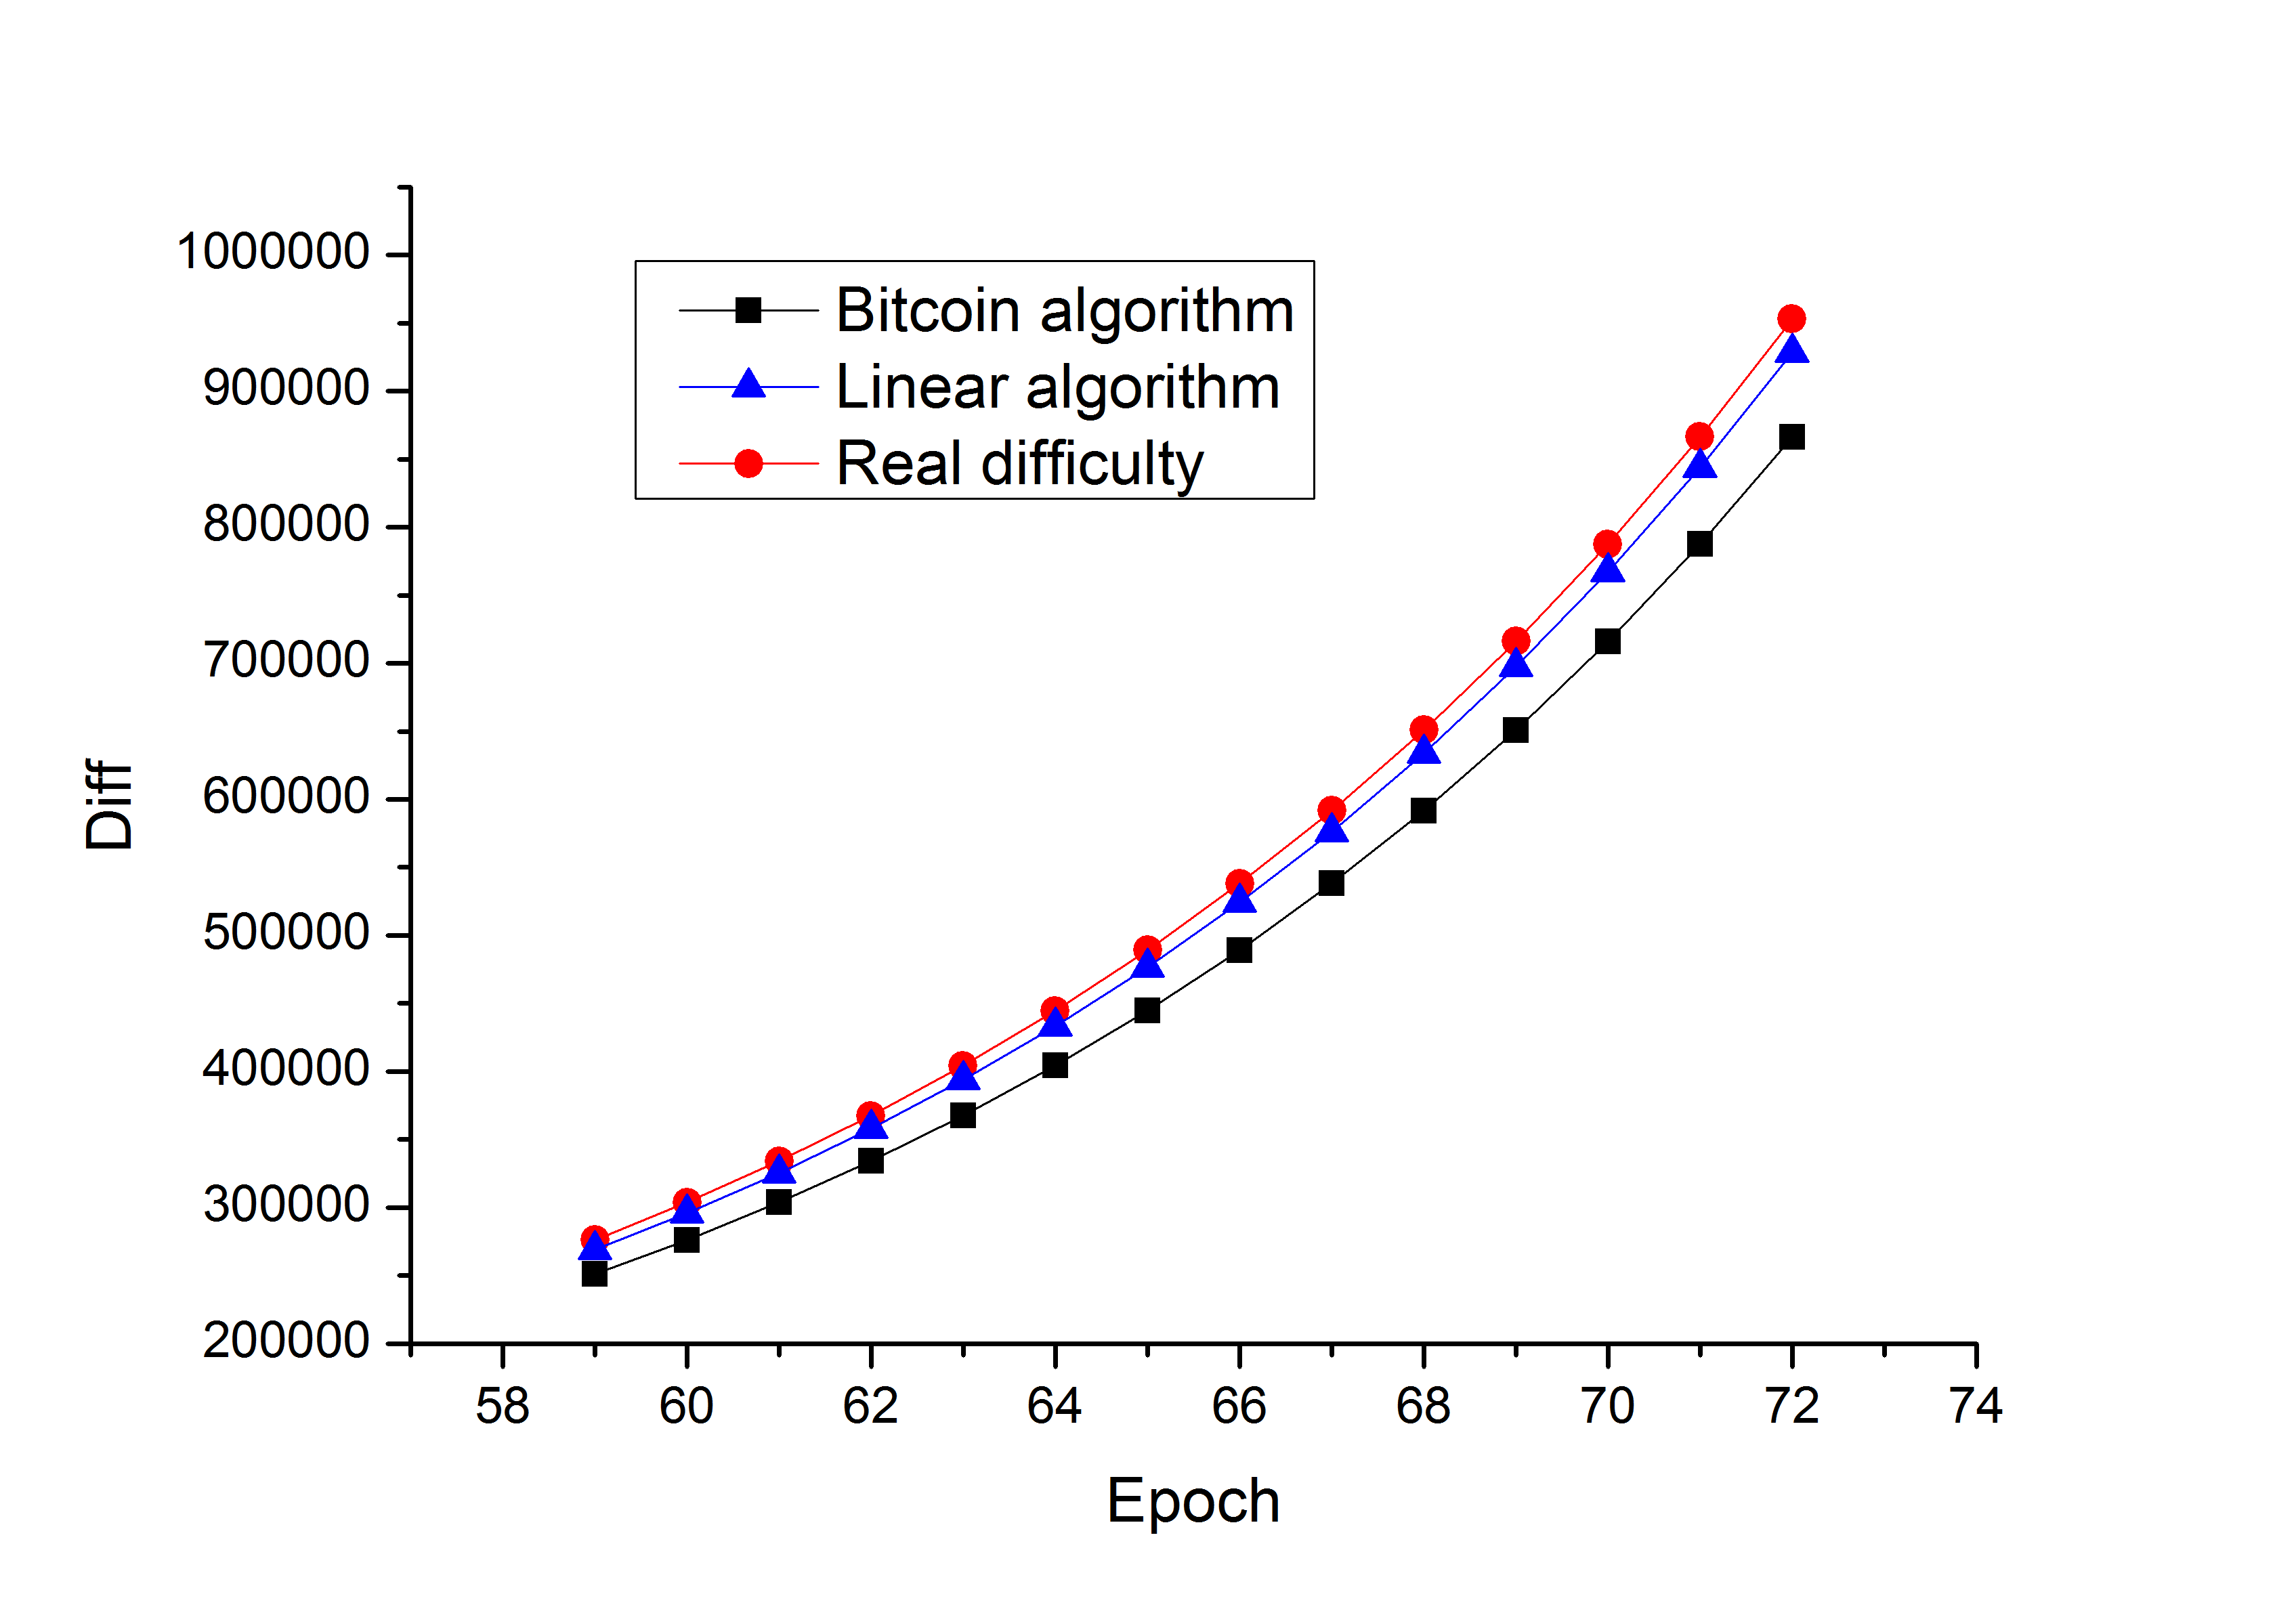
\includegraphics[scale=0.3]{exp.png}}
\caption{Real difficulty (red) and difficulties calculated from Bitcoin (black) and linear (blue) algorithms in situation of exponential hash rate growth}
\label{fig:exp}
\end{figure}

Note that the difficulty calculated from Bitcoin algorithm is always significantly lower than the real one.
This leads to a {\em 9 min 5 sec} time interval between blocks, which is $\approx$10\% lower then desired {\em 10 min} interval.
Difficulty calculated by the linear algorithm is also aways lower than the real one, but closer to it.
Mean delay between blocks when linear algorithm is used is {\em 9 min 45 sec}, which is closer to the planned value. The algorithm currently used in the Bitcoin network has an average error of about 9.1\%, while our algorithm has an error of about 1.9\%.

While the difficulty update algorithm, proposed in~\cite{kraft2015difficulty} leads to better results for exponential difficulty growth with a constant rate, we note that our algorithm is much simpler and may be implemented with integer arithmetic only.
%Moreover, exponential difficulty growth is the simplification of the difficulty growth law, and it may be incorrect to expect it in some situations.

\subsection{Real World Data}

We compare the real Bitcoin network data with difficulty values calculated by the algorithm used in Bitcoin. Furthermore, we do the same with values calculated by the linear algorithm. %Results are shown in figure~\ref{fig:real_world_difficulty}.

%\begin{figure}[h]
%\center{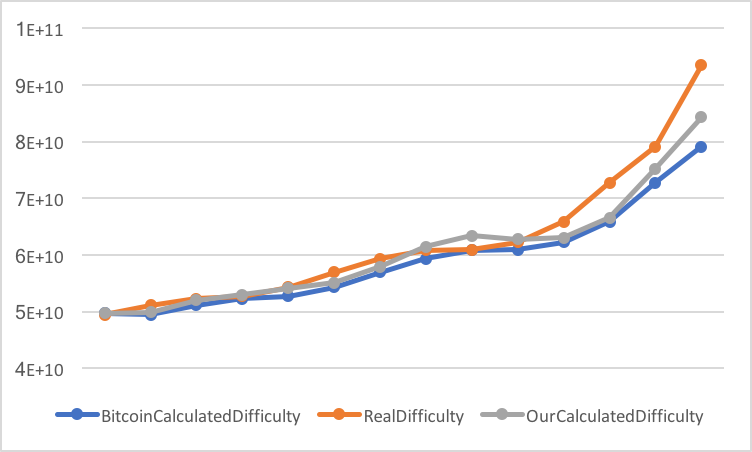
\includegraphics[scale=0.5]{real_world_difficulty.png}}
%\caption{Comparison of the real world difficulty data from the Bitcoin network}
%\label{fig:real_world_difficulty}
%\end{figure}

Results show that in average Bitcoin algorithm has an error of about 12.3\% while our approach only has an error of about 8.4\%. Thus  our approach performs about 33\% better than the approach currently used in the Bitcoin network.

\subsection{\AttackName}

We consider the \attackname{} as described in the Section~\ref{sec:attack}: an attacker with computational power \(R_a\) (for simplicity we suppose \(R_a=0.2 \cdot R_0 \) in this section) turn on and turn off his mining to manipulate difficulty and produce more blocks.
Figure \ref{fig:attack} represents difficulty over epochs for this scenario.

\begin{figure}[h]
\center{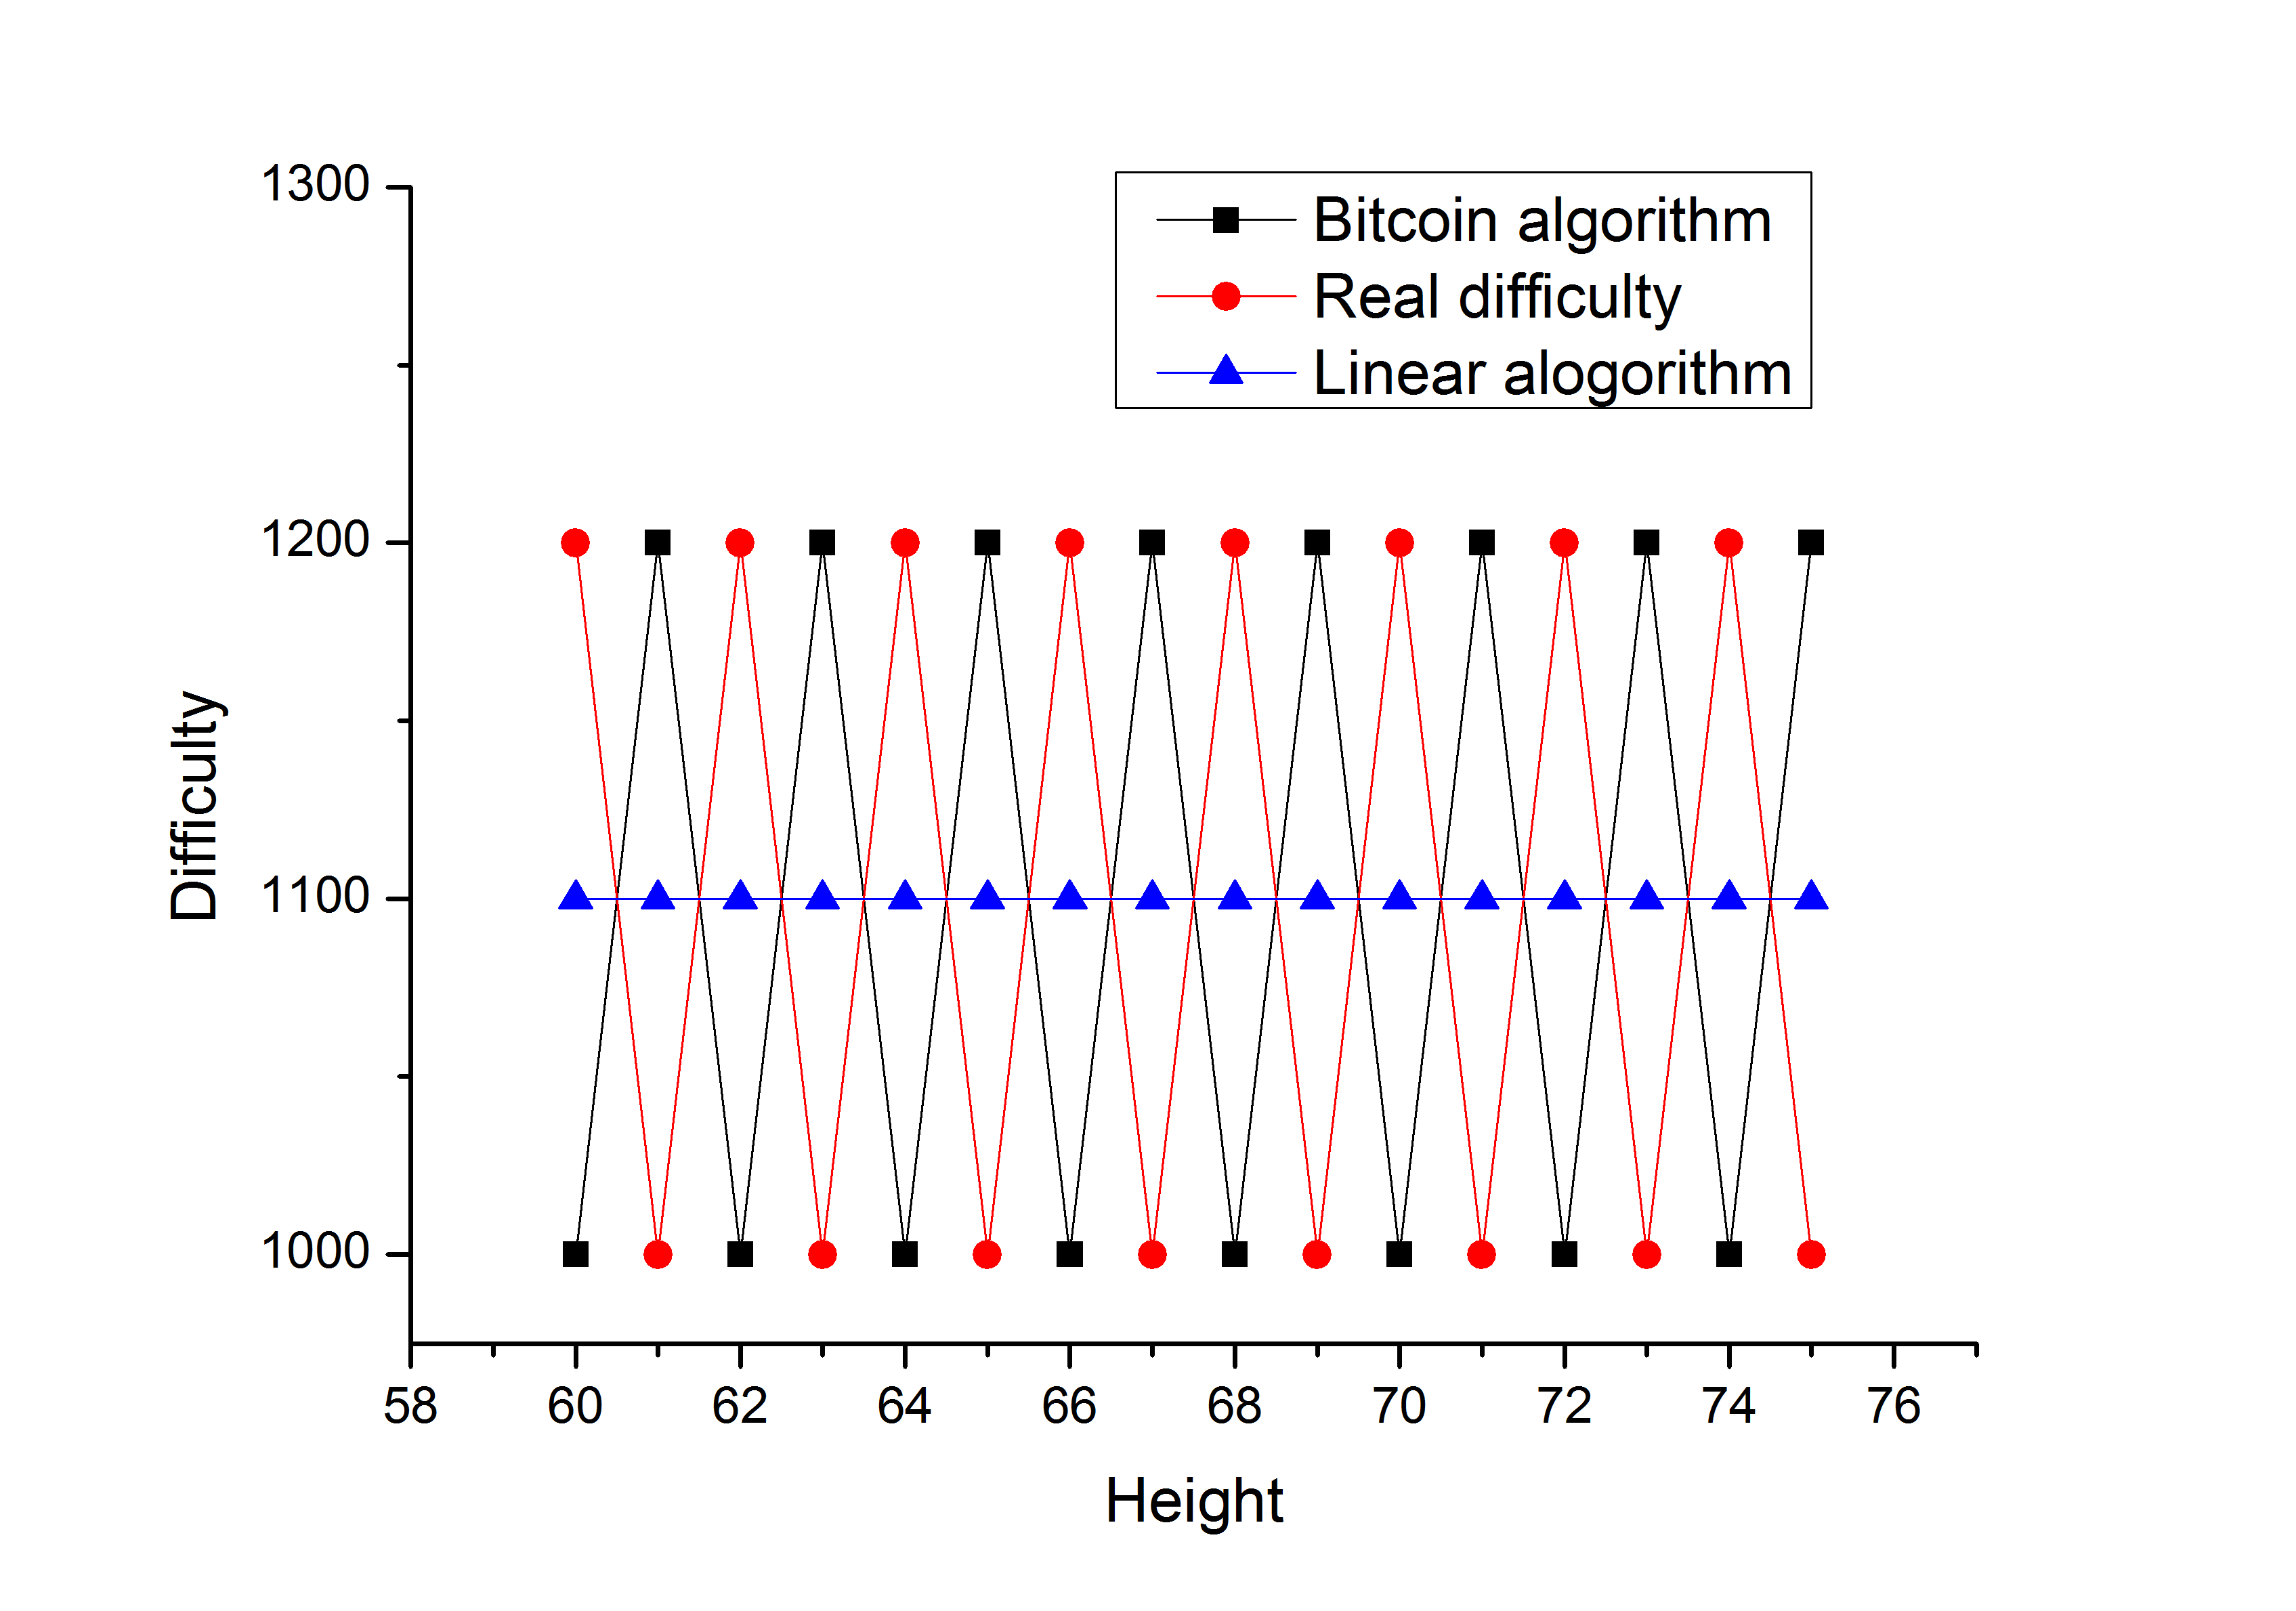
\includegraphics[scale=0.3]{attack.png}}
\caption{Real difficulty (red) and difficulties calculated from Bitcoin (black) and linear (blue) algorithms in \attackname{}}
\label{fig:attack}
\end{figure}

Note that the difficulty calculated with the Bitcoin algorithm is always in antiphase with the real one.
The Bitcoin difficulty update algorithm leads to {\em 10 min 10 sec} mean delay between blocks, which is in good correlation with the Equation~\ref{eq:ati}.
The linear algorithm also leads to bigger than planned mean delay between blocks of {\em 10 min 5 sec}, which is about two times lower divergence in comparison with the algorithm of Bitcoin. Obviously, the profit of the attacker is then also 2 times lower, which is a serious improvement.

Thus the linear difficulty control algorithm, proposed in Section \ref{sec:improved} is better than the one used in Bitcoin for the \attackname{} scenario, both in terms of block rate and attacker's profit.



%\section{Conclusion}
%\label{sec:concl}
%In this paper we analyze a new kind of attacks on the blockchain based on manipulating mining difficulty. This attack decreases computational power spent by an attacker for block mining while increasing mean time interval between blocks. It is especially favorable in situation, when the cost of computational resources invested into mining is around the expected reward and there are enough forks to switch mining between them.

%To improve the stability of block times and decrease the attacker profit, we proposed an alternative difficulty update algorithm, based on linear regression. It was found that this algorithm performs better then the one used in Bitcoin both in terms of block rate and in terms of attacker profit, while it's still simple enough to be computed with integer arithmetic only.

%\section*{Acknowledgments}

\bibliographystyle{elsarticle-num}
\bibliography{sources.bib}


\end{document}